\documentclass[a4paper,12pt]{report}
\usepackage[english]{babel}
\usepackage{subcaption}
\usepackage{amsmath}
\usepackage{amssymb}
\usepackage{amsthm}
\usepackage{float} 
\usepackage{lscape}
\usepackage{array}
\usepackage[matrix,arrow,curve]{xy}
\usepackage[T2A]{fontenc}
\usepackage[cp1251]{inputenc}
\usepackage{graphicx}
\usepackage{makecell}
\usepackage{titlesec}
\usepackage{titletoc}
\usepackage{blkarray}
\usepackage{rotating}
\usepackage{longtable}
\usepackage{geometry}
\usepackage{fancyhdr}
\usepackage{enumitem}
\newlist{steps}{enumerate}{1}
\setlist[steps, 1]{label = Step \arabic*:}
\usepackage{diagbox} 
\usepackage{multirow}
\usepackage{url}
\usepackage{gensymb}

\usepackage{bookmark}
\usepackage[]{hyperref}
\hypersetup{hidelinks} % removes squares from hyperlinks

% \textwidth=175mm  \textheight=257mm
% \voffset=-2.64cm  \hoffset=-1.85cm
\geometry{tmargin=2cm,bmargin=2cm,lmargin=2.5cm,rmargin=1cm}

\fancyhf{}
\renewcommand{\headrulewidth}{0pt}
\fancyhead[C]{\thepage}
\pagestyle{fancy}
\fancypagestyle{plain}{%
  \fancyhf{} % clear all header and footer fields
  \renewcommand{\headrulewidth}{0pt}
  \fancyhead[C]{\thepage} % except the center
}
\setlength{\headheight}{35pt}

\renewcommand{\thesection}{\arabic{chapter}.\arabic{section}}
\renewcommand{\thesubsection}{\arabic{chapter}.\arabic{section}.\arabic{subsection}}

\titleformat{\chapter}[display]{\bf\Huge\filcenter}{\chaptername\,\,\thechapter}{.5em}{}{}
\titlecontents{chapter}[0pt]{\filright}{\bf\chaptername\,\,\thecontentslabel \ }{\bf}{\dotfill\thecontentspage}
%\titleformat{\section}[block]{\bf\Large\filcenter}{\sectionname\,\,\thesection}{.5em}{}{}
\titlecontents{section}[1em]{\filright}{\thecontentslabel \ }{}{\dotfill\thecontentspage}
%\titleformat{\subsection}[block]{\bf\large}{\subsectionname\,\,\thesubsection}{.5em}{}{}
\titlecontents{subsection}[2em]{\filright}{\thecontentslabel \ }{}{\dotfill\thecontentspage}

\usepackage{xcolor,paracol}
\setlength{\parindent}{15pt}
\setcounter{page}{1} 
\renewcommand{\baselinestretch}{1.2}
\newtheorem{acknowledgement}{Acknowledgement}

\newtheorem{definition}{Definition}[chapter]
\newtheorem{lemma}{Lemma}[chapter]
\newtheorem{theorem}{Theorem}[chapter]
\newtheorem{remark}{Remark}[chapter]
\newtheorem{proposition}{Proposition}[chapter]
\newtheorem{property}{chapter}
\newtheorem{corollary}{Corollary}[chapter]
\newtheorem{assumption}{Assumption}[chapter]
\newtheorem{example}{Example}[chapter]

\renewcommand{\thesection}{\arabic{chapter}.\arabic{section}}
\renewcommand{\theequation}{\arabic{chapter}.\arabic{equation}}
\newcommand{\secref}[1]{\S\ref{#1}}
\renewcommand*\footnoterule{}
\begin{document}
\thispagestyle{empty}
\begin{center}
{\textbf{Stellenbosch University}}\\
\vskip 20pt

\begin{flushleft}
\hskip 320pt { 
Contract number: S008856
}
\end{flushleft}
\vskip 90pt
{\textbf{\Large }}\\
\vskip 60pt
{\LARGE \textbf{
Enaex Robotics in Mining}}\\
\vskip 25pt
\textbf{\large Research Chair}\\
\vskip 40pt
\textbf{\Large Project notes} \\
\vskip 40pt
Department of Electrical and Electronics Engineering \\
\vskip 60pt
\begin{flushleft}
\hskip 350pt {\Large PI:
}\\
\vskip 5pt
\hskip 350pt {\Large Dr.}\\
\vskip 5pt
\hskip 350pt {\Large Callen Fisher}
\end{flushleft}
\vskip 100pt

Stellenbosch University\\
\vskip 10pt
2024 to 2026
\end{center}

\vfil\eject

\large  \tableofcontents
\renewcommand{\partname}{Chapter}

\chapter{Component Comparisons}
%\addcontentsline{toc}{chapter}{Introduction}\label{Introduction}

In this section different component of the drone will be discussed. The components discussed are those involved in the construction of the basic drone, before any mine specific sensors are added.

\section{Frame}
	Frame
	\begin{itemize}
		\item Source One V5: Affordable, open-source, compatible with latest hardware, large collection of spare parts, mods and accessories ("check Thingyverse website"), 123.5g
		\item AOS 5 V2: FPV performance focussed, exceptional noise performance and prop wash handling, complex building and repairing, arms are prone to damage during crashes, 125g
	\end{itemize}

	Final Decision: Source One V5
	
\section{Motors and Propellers}
	\subsection{Motor Considerations}
		\begin{itemize}
			\item Lower KV ratings for better efficiency
			\item Larger LiPo or Li-ion Batteries
		\end{itemize}

	\subsection{Propeller Considerations}
		\begin{itemize}
			\item Lower pitch propeller for better efficiency
			\item 5" = smaller, 7" more payload and better efficiency
			\item Therefore 6" might be optimal? but check availability?
		\end{itemize}
	
	Combining these meanings, ``OreHawk'' could suggest a project or initiative that involves a vigilant and focused approach to monitoring, extracting, or managing valuable minerals or resources in the mining industry. The name implies a keen eye for detail and a strategic, purposeful effort in dealing with ore-related activities.


\section{Electric Speed Controller (ESC)}
	Some of the basic requirements are:
	\begin{itemize}
		\item Fully electric
		\item under 1m in height
		\item Fully autonomous
		\item must map and scan the area (see objectives)
		\item Must be able to identify misfires and remove them
		\item Must be able to predict the direction of the reef
		\item Must map the holes and pass on the info to a secondary robot
		\item Must set up a comms network
		\item Battery life of 8 hours
		\item Must be able to scan two stope faces in the 8 hours
		\item 
	\end{itemize}
	
\section{Flight Controller/Autopilot}

	\begin{enumerate}
		\item Map the area
		\item Map the stope face
		\begin{enumerate}
			\item Surface map
			\item Reef map
		\end{enumerate}
		\item Scan and map drilled holes
		\begin{enumerate}
			\item Accurately map position, depth and angle of hole
			\item Scan emulsion in hole (replace cup test)
			\item Scan for misfires
		\end{enumerate}
		\item Remove misfires
		\item Program detonators
		\item Transmit all data to base station
	\end{enumerate}

\section{Details of the environment}
	During one of my visits to Impala Platinum mines, several photos of the environment was captured and shown below. Please note these images should not be shared, however, we can potentially use them in your dissertations. 
	
	Some notes on the environment:
	
	\begin{itemize}
		\item Extremely rough terrain
		\item The reef is less than 1m in height, so the robot has to be quite compact
		\item The ground has the texture of a fine paste that has Chrome in it, so it will grind away at any moving parts. 
		\item There are tons of objects in the way, these range from support pillars, roof bolts, cables, discarded things etc
		\item The temperature and humidity is very high
		\item There is lots of particle matter in the air
		\item It is very dark
		\item 
	\end{itemize}

	Here are some of the images I have and a description of them:

	\begin{figure}[H]
		\centering
		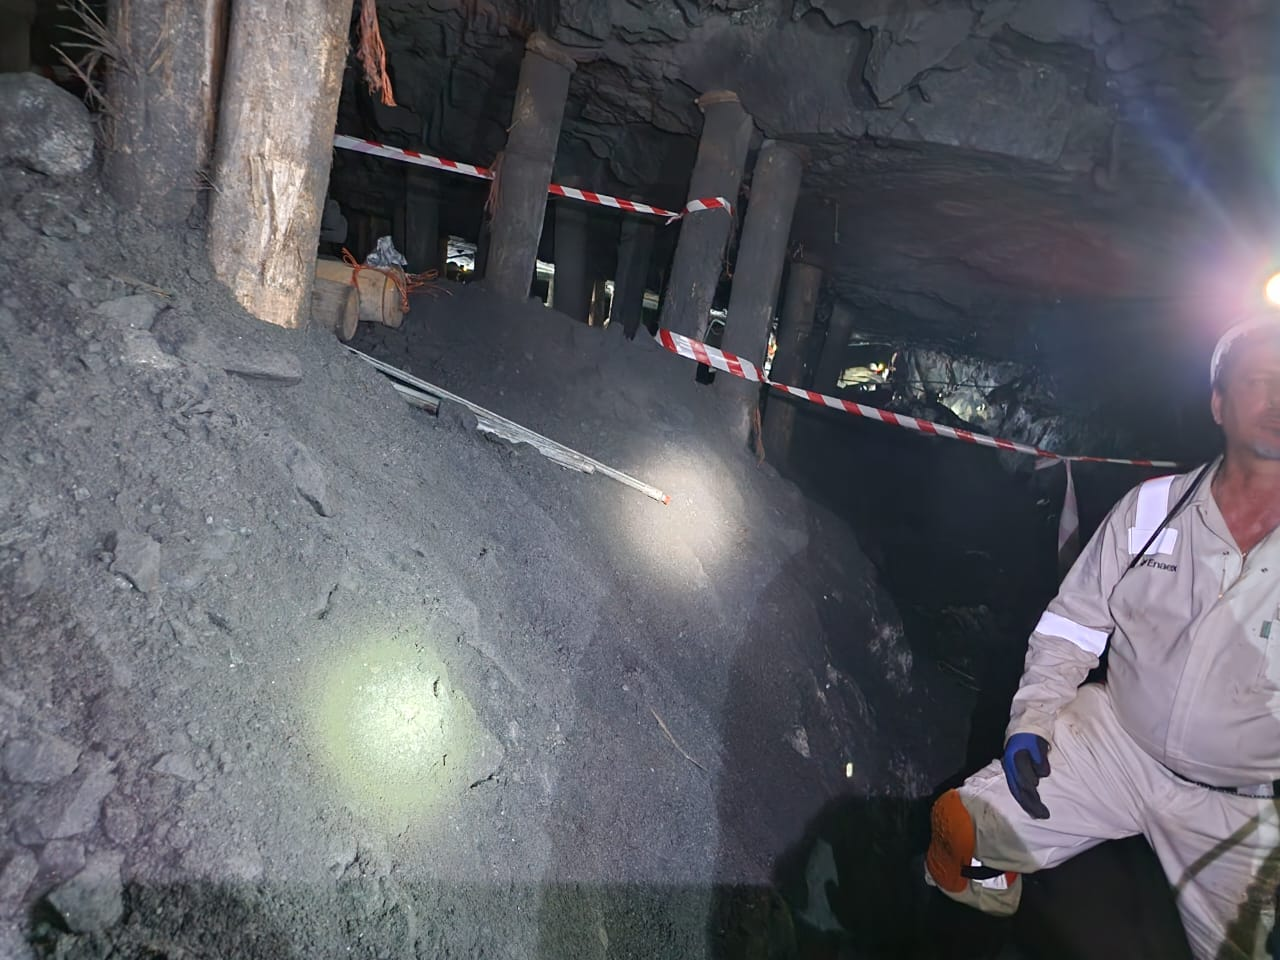
\includegraphics[width=0.7\linewidth]{Images/Impala1}
		\caption{Impala platinum mine. Person for scale, on the left is the narrow reef, which is less than 1m in height. Note the rise between the walkway and the reef that is being mined. The wooden pillars are there to support the roof.}
		\label{fig:Impala1}
	\end{figure}

	\begin{figure}[H]
		\centering
		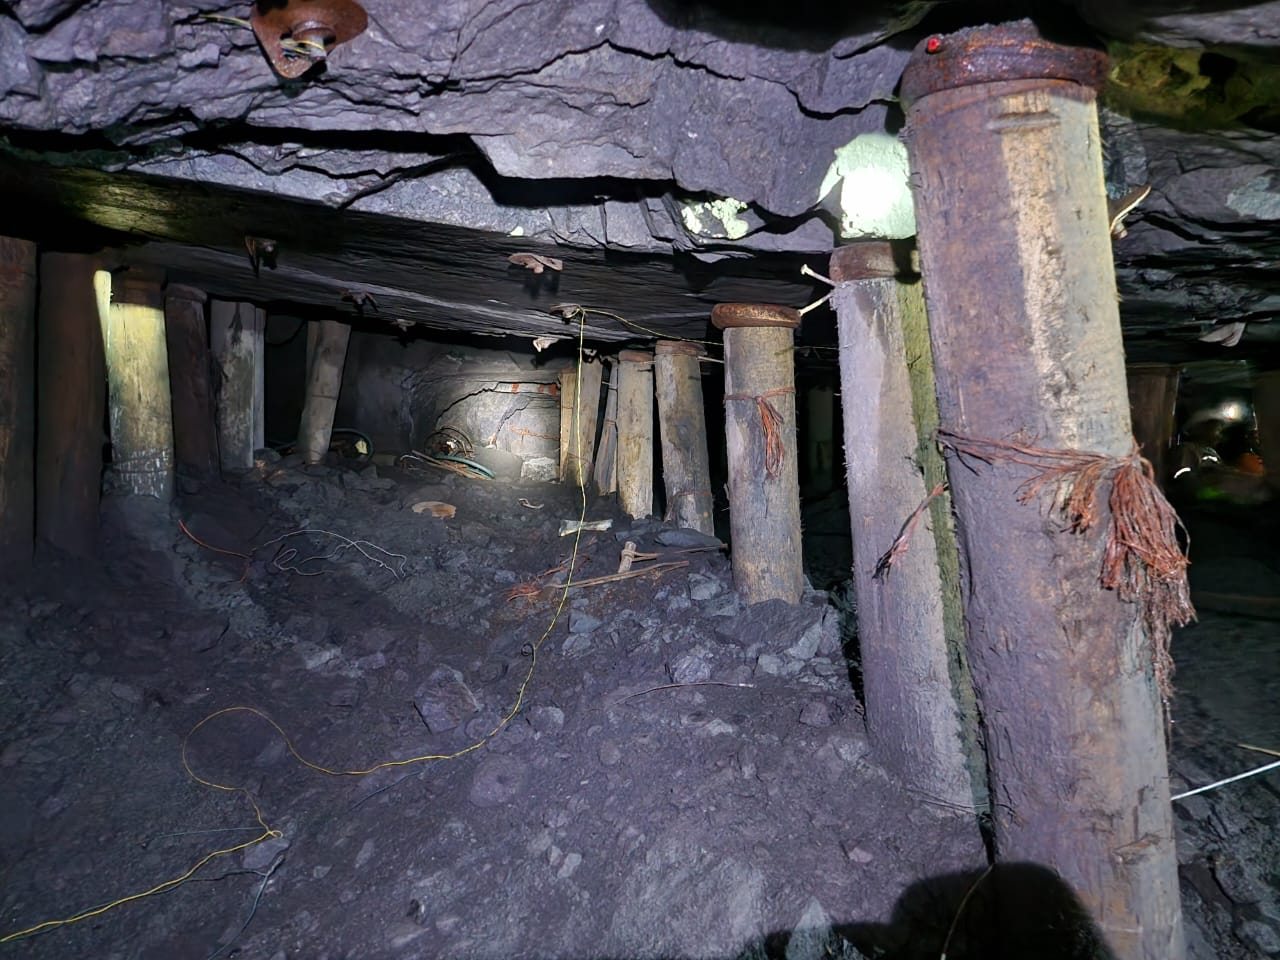
\includegraphics[width=0.7\linewidth]{Images/Impala2}
		\caption{Impala platinum mine. An image of the reef that has been mined. If you look at the top left of the image, there is a roof bolt sticking out. Note the roughness of the mined area, the vehicle will have to travel through this. Note how there are also wires and other things in the way. Nothing is smooth.}
		\label{fig:Impala2}
	\end{figure}

	\begin{figure}[H]
		\centering
		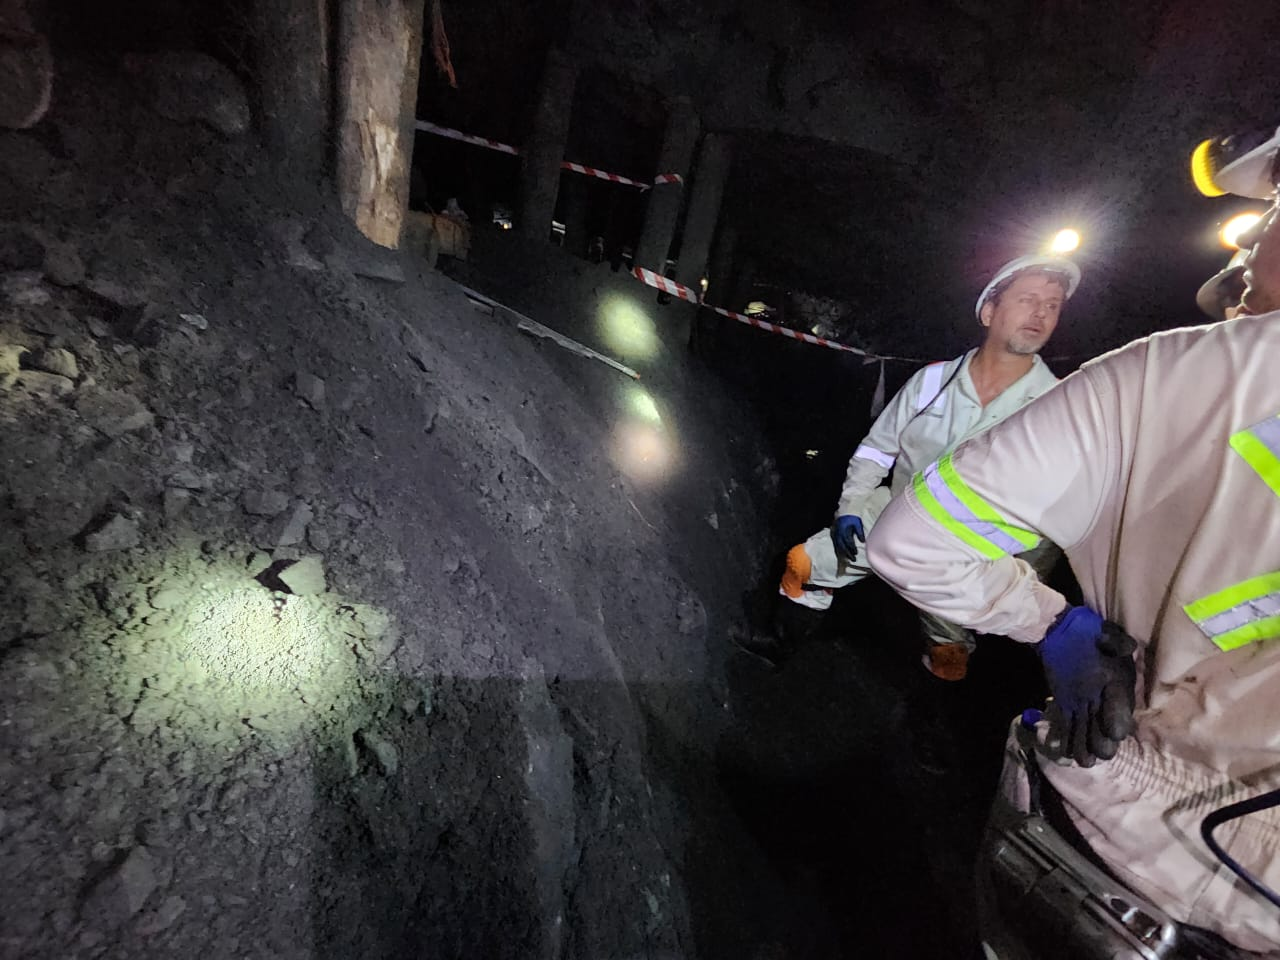
\includegraphics[width=0.7\linewidth]{Images/Impala3}
		\caption{Impala platinum mines. Notice the step up between the walkway and the reef. There will be a scissor lift to raise the robot to the reef. Again, look at the ground surface. It is almost like a grinding paste with Chrome in it, that will wear away any moving parts. }
		\label{fig:Impala3}
	\end{figure}
	
	\begin{figure}[H]
		\centering
		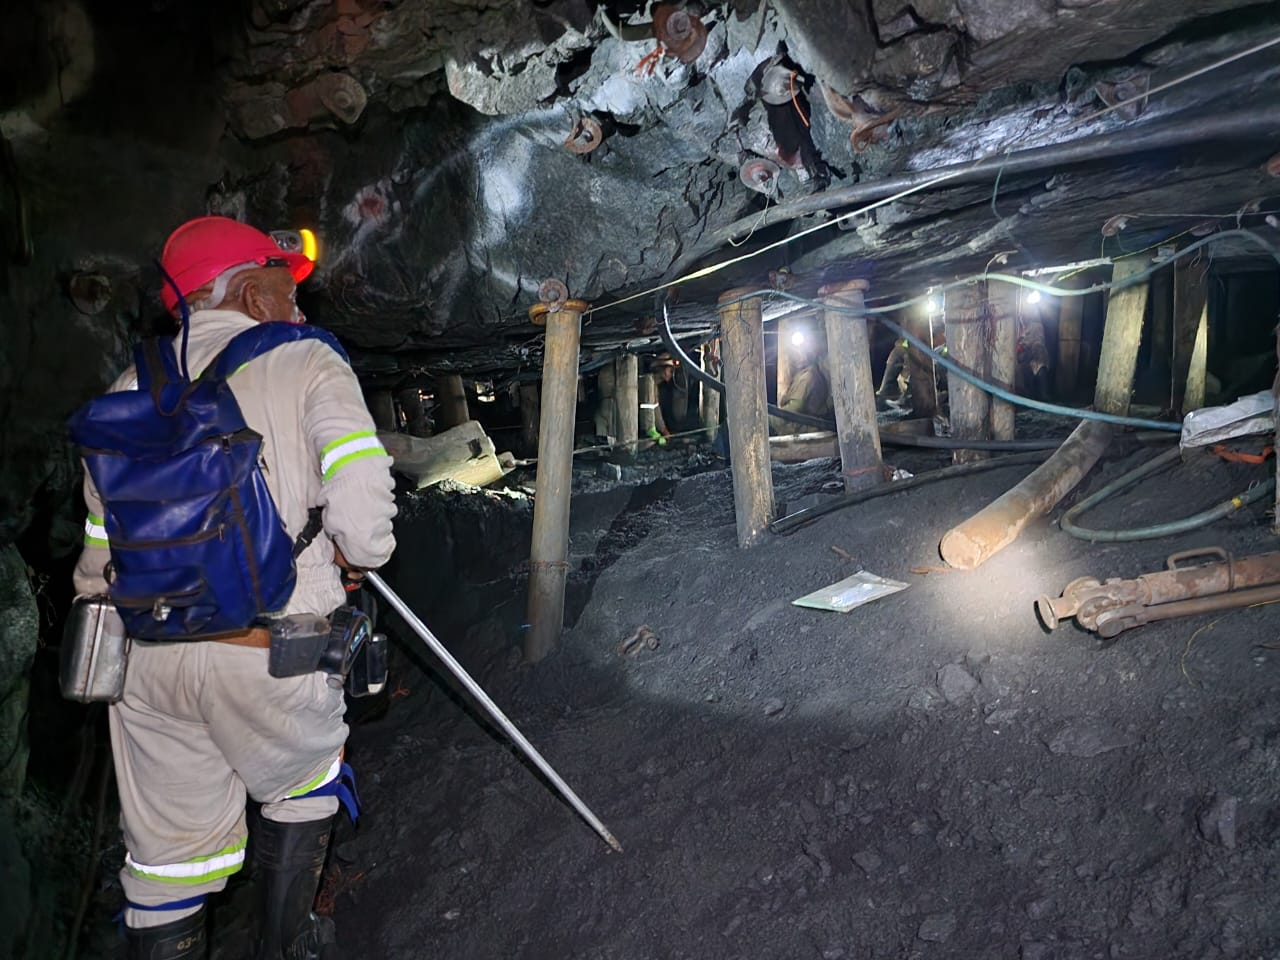
\includegraphics[width=0.7\linewidth]{Images/Impala4}
		\caption{Impala platinum mine. Person for scale. Notice all the cables, the roughness of the roof and all the obstacles in the way of the robot.}
		\label{fig:Impala4}
	\end{figure}
	
	\begin{figure}[H]
		\centering
		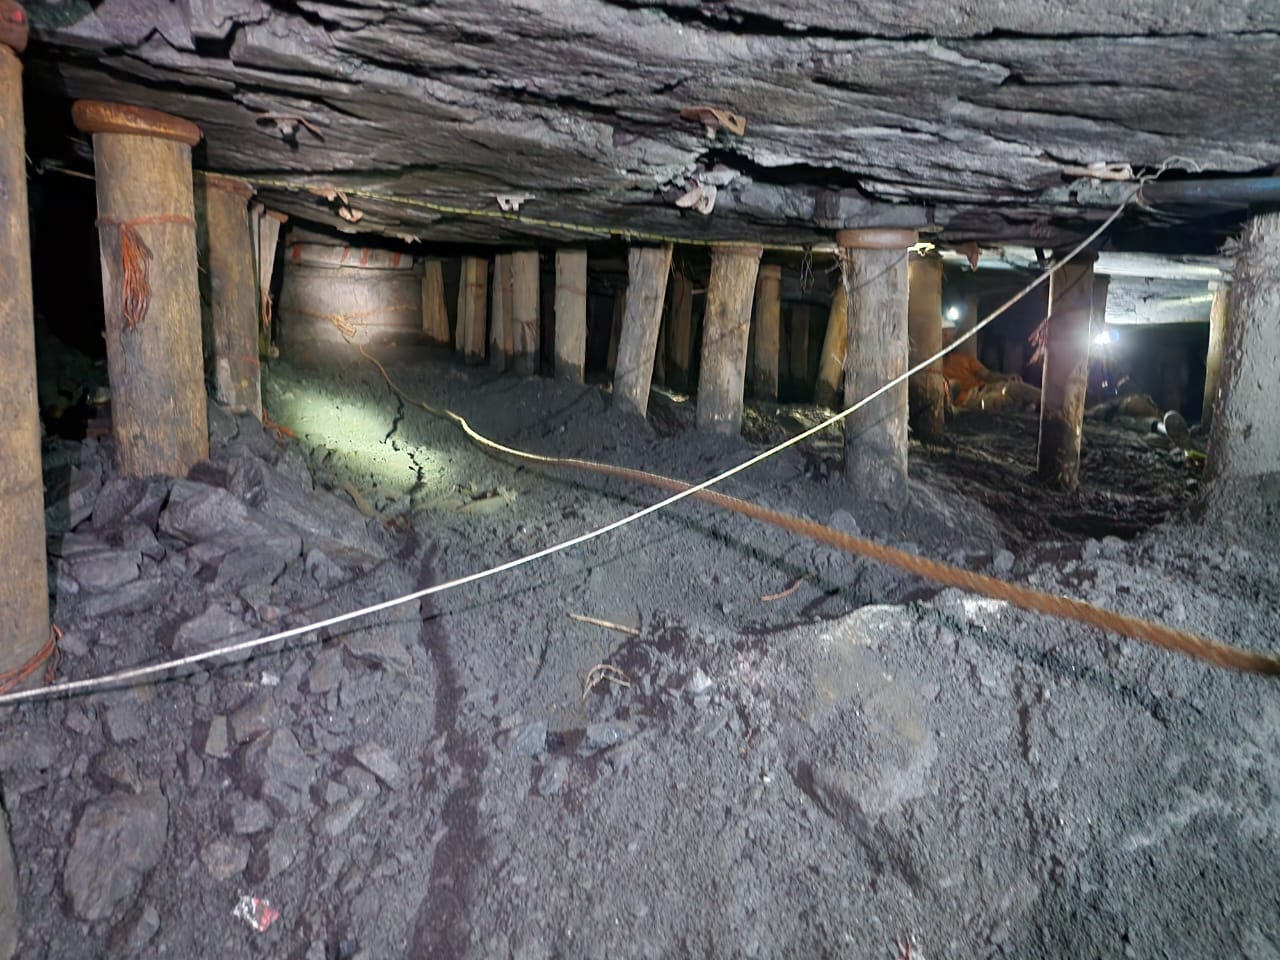
\includegraphics[width=0.7\linewidth]{Images/Impala5}
		\caption{Impala platinum mine. Notice the people sitting in the background for scale. }
		\label{fig:Impala5}
	\end{figure}
	
	\begin{figure}[H]
		\centering
		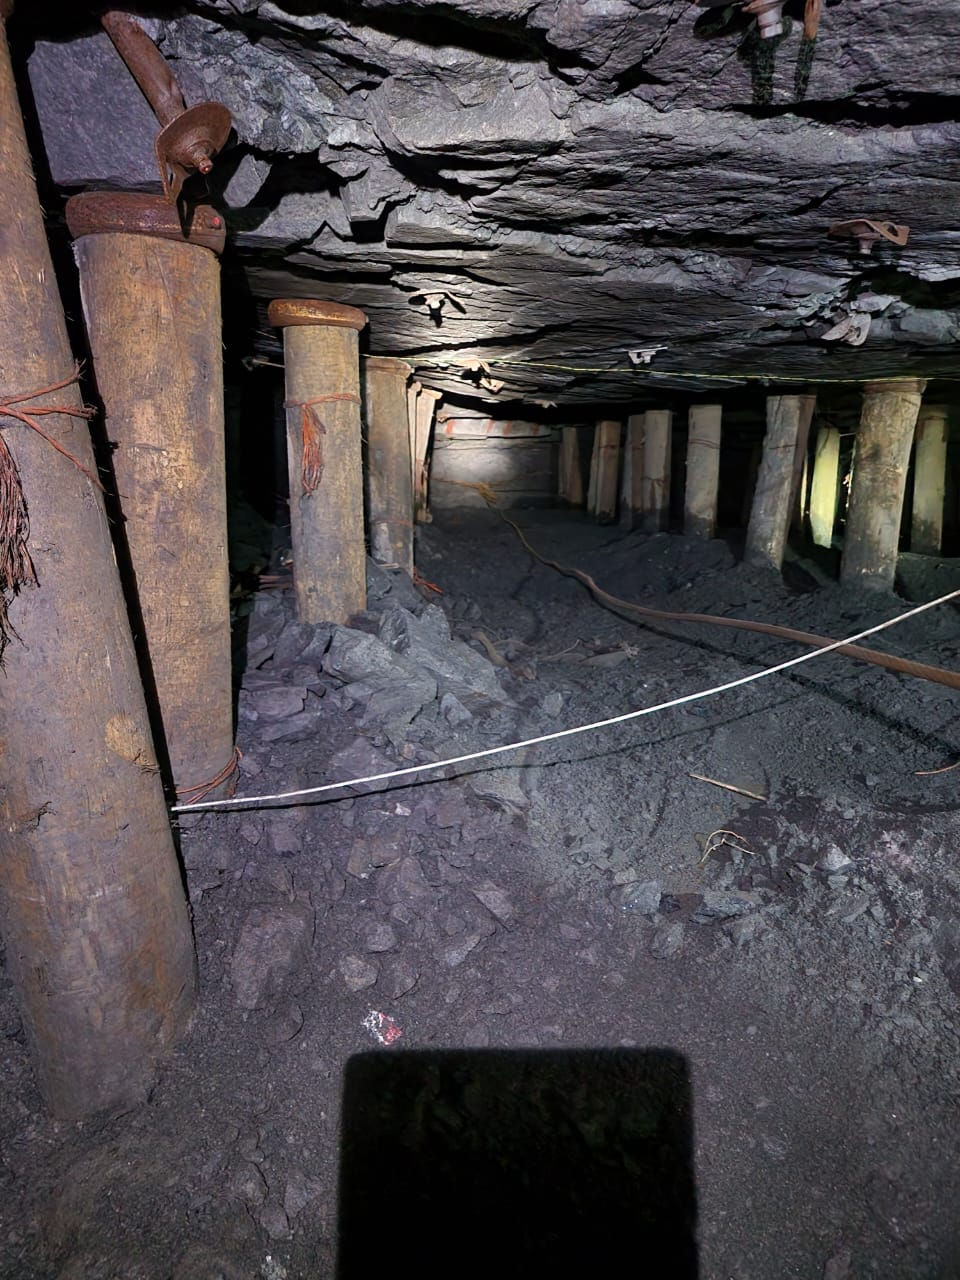
\includegraphics[width=0.7\linewidth]{Images/Impala6}
		\caption{Impala platinum mines. Notice the roof bolts}
		\label{fig:Impala6}
	\end{figure}
	
\section{Specifications of stope face}
	
	\subsection{Stope Face specifications}
		\begin{itemize}
			\item Length: 15m? 
			\item Height: 900mm
			\item Number of holes: 150
			\item 
		\end{itemize}
		
	\subsection{Hole specifications}
		\begin{itemize}
			\item Diameter: 38mm $\pm$ 3mm
			\item Depth: 2000mm to 2200mm
			\item Max angle: 0 to 15 degrees
			\item Distance from roof to hole: 150mm to 200mm
			\item Distance from floor to hole: 150mm to 200mm
			\item 
		\end{itemize}
		
	\subsection{Terrain and environment specifications}
		\begin{itemize}
			\item Slope: 12 degrees
			\item Maximum obstacle size: 100mm
			\item Particle matter: $1.88MG/M^3$
			\item Temperature:28-32 degrees Wet bulb
			\item Duration of operation:
			\item Lift platform: 2.3m by 8m
		\end{itemize}
	
\section{Project plan and timeline}

	\subsection{Year 1 (2024)}
		\begin{itemize}
			\item Field test handheld scanner
			\item Build the rover
			\item Basic navigation and mapping
		\end{itemize}

	\subsection{Year 2 (2025)}
		\begin{itemize}
			\item 3rd person view on a tablet
			\item Advanced navigation of cluttered environment
			\item Navigation of rough terrain
			\item Advanced mapping of mine/tunnel
		\end{itemize}

	\subsection{Year 3 (2026)}
		\begin{itemize}
			\item System integration
			\item Comms problem solved
			\item Advanced navigation of rough terrain
			\item Test in mine
			\item Robotic arm control
			\item Mapping of holes
			\item Mapping of reef
		\end{itemize}

\section{Testing methodology}
	The goal is to rapidly test and prototype everything. As we develop something small we need to test it, film it and document it. Enaex is all about ``Fail fast'', where we need to try things as soon as possible to see if they will work, as soon as they don't work, pivot and try something else.
	
	There are several caves and abandoned mines and tunnels in the mountains around Cape Town and Stellenbosch. I will go explore some in the coming months. These will be used as initial environments to test these sensors and prototypes. 
	
	Once we have a working prototype, I can investigate testing in an active mine shaft in Johannesburg, this will obviously be very time consuming and expensive, so we have to thoroughly test these devices first, to ensure a successful test.  

	Make sure that every test is well documented and backed up. This will make writing up your thesis much easier, as you wont have to repeat any early day tests. Make sure all the data and images are of good quality for the final report, even if you do not end up using the test. 
	
	Additionally, if something goes wrong (lost robot, broken PC, etc) you have initial data and results that you can use to add to your report. I have had students that have lost almost all their data before a submission, resulting in a sub-par mark where their research deserved a much higher mark. 
\section{Common sensor pack}
	This project will consist of several robotic platforms:
	
	\begin{itemize}
		\item Main rover
		\item Rover test platforms (RC cars, etc)
		\item Drones
		\item Handheld scanner
	\end{itemize}
	
	It is crucial that we stick to a common sensor architecture. Obviously, the drones will have fewer sensors due to their payload capacity, however the other platforms must stick to the same sensors. This way our code becomes independent of the platform. Some platforms might have fewer sensors, but the sensors they do have must be the same (for example, if you use an RGB-D camera, it must be the same camera used on all the other platforms).
	
	Therefore, it is crucial to pick the correct sensors from day one! We will do a thorough literature review and component comparison before we purchase anything. 


\section{Conferences:}
	We need to publish continuously. There are several conferences coming up that we need to try aim for:
	
	\begin{itemize}
		\item RobMech: Very weak conference\\
		Due date:
		\item CCA24: Very weak conference\\
		Due date: 
		\item ICRA: Top robotics conference\\
		Due date:
		\item IROS: Top robotics conference\\
		Due date:
	\end{itemize}




























\vfil\eject

\chapter{Final Component Selection}

The following table gives the final list of components selected for the drone construction. The list also includes the prices of the coponents and the approximate mass.

\begin{table}[H]
	\begin{center}
		\begin{tabular}{|l|l|l|l|l|}
		\hline
		Component              & Component Selected               & Price/unit (R)    & Mass (g)          & Import ? \\ \hline
		Frame                  & TBS Source One V5 5inch (US\$30) & $\sim$600         & 123.5             & Yes      \\
		Motors                 &                                  &                   &                   &          \\
		Propellers             &                                  &                   &                   &          \\
		Electronic Speed       & \multirow{2}{*}{}                & \multirow{2}{*}{} & \multirow{2}{*}{} &          \\
		Controller (ESC)       &                                  &                   &                   &          \\
		Flight Controller /    &                                  &                   &                   &          \\
		Autopilot              &                                  &                   &                   &          \\
		Microcontroller        &                                  &                   &                   &          \\
		Power Distribution     &                                  &                   &                   &          \\
		Board (PDB)            &                                  &                   &                   &          \\
		Battery                &                                  &                   &                   &          \\
		Battery Charger /      &                                  &                   &                   &          \\
		Balance Charger        &                                  &                   &                   &          \\
		Voltage Sensor         &                                  &                   &                   &          \\
		and Regulator          &                                  &                   &                   &          \\
		Communications Antenna &                                  &                   &                   &          \\
		\& Remote Controller   &                                  &                   &                   &          \\ \hline
		\end{tabular}
	\end{center}
\end{table}

\vfil\eject

\chapter{Interesting Additional Components to Investigate}

A place where I add random ideas or notes that we should consider. Please remove once they have been dealt with:


\section{Nico}
	\begin{itemize}
		\item Full frame not needed, do not want to block the camera/lidar view \cite{RMFOwl}
		\item Aiming to support the goal of autonomous exploration in diverse subterranean settings \cite{RMFOwl}
		\item Make a resilient micro flyer
		\item Use mini drones for full local map completion \cite{GraphBased}
		\item ``mother'' and ``baby'' robot, which is released to map hard to acess areas \cite{DarpaMultiRobot}
		\item valid option to provide rapid situational awareness to a small team of operators prior to possible entry in such unknown and dynamic areas \cite{Cerberus}
		\item aerial scouts \cite{Cerberus}
		\item Flying robots were the complimentary system to fill the gap and explore highly vertical environments and impassable terrain. \cite{Cerberus}
	\end{itemize}

\section{Hansie}
	\begin{itemize}
		\item Provide rapid situational awareness to a team of operators \cite{DarpaSynopsis}
		\item Tethered robot and deployable nodes \cite{Cerberus}
	\end{itemize}

\section{Adam}
	\begin{itemize}
		\item 
	\end{itemize}	
\vfil\eject

% \chapter*{Bibliography}
\addcontentsline{toc}{chapter}{Bibliography}

\begin{thebibliography}{99}

    \bibitem{compSLAM} Khattak, Shehryar, et al. "Complementary multi–modal sensor fusion for resilient robot pose estimation in subterranean environments." 2020 International Conference on Unmanned Aircraft Systems (ICUAS). IEEE, 2020.



	\bibitem{RMFOwl} De Petris, Paolo, et al. ``Rmf-owl: A collision-tolerant flying robot for autonomous subterranean exploration.'' 2022 International Conference on Unmanned Aircraft Systems (ICUAS). IEEE, 2022.
	
	\bibitem{CoSTAR}Otsu, Kyohei, et al. ``Supervised autonomy for communication-degraded subterranean exploration by a robot team.'' 2020 IEEE Aerospace Conference. IEEE, 2020.
	
	\bibitem{LAMP} Ebadi, Kamak, et al. ``LAMP: Large-scale autonomous mapping and positioning for exploration of perceptually-degraded subterranean environments.'' 2020 IEEE International Conference on Robotics and Automation (ICRA). IEEE, 2020.
	
	\bibitem{GraphBased} Dang, Tung, et al. ``Graph-based path planning for autonomous robotic exploration in subterranean environments.'' 2019 IEEE/RSJ International Conference on Intelligent Robots and Systems (IROS). IEEE, 2019.
	
	\bibitem{ExploreLocally} Dang, Tung, et al. ``Explore locally, plan globally: A path planning framework for autonomous robotic exploration in subterranean environments.'' 2019 19th International Conference on Advanced Robotics (ICAR). IEEE, 2019.
	
	\bibitem{GazeboCave} Koval, Anton, et al. ``A subterranean virtual cave world for gazebo based on the DARPA SubT challenge.'' arXiv preprint arXiv:2004.08452 (2020).
	
	\bibitem{HeterogeneousSystem} Biggie, Harel, and Steve McGuire. ``Heterogeneous Ground-Air Autonomous Vehicle Networking in Austere Environments: Practical Implementation of a Mesh Network in the DARPA Subterranean Challenge.'' 2022 18th International Conference on Distributed Computing in Sensor Systems (DCOSS). IEEE, 2022.
	
	\bibitem{DarpaSynopsis} Orekhov, V., and T. Chung. ``The DARPA subterranean challenge: A synopsis of the circuits stage.'' Field Robotics 2.1 (2022): 735-747.

	\bibitem{DarpaMultiRobot}Rouček, Tomáš, et al. ``Darpa subterranean challenge: Multi-robotic exploration of underground environments.'' Modelling and Simulation for Autonomous Systems: 6th International Conference, MESAS 2019, Palermo, Italy, October 29–31, 2019, Revised Selected Papers 6. Springer International Publishing, 2020.
	
	\bibitem{Cerberus} Tranzatto, Marco, et al. ``CERBERUS in the DARPA Subterranean Challenge.'' Science Robotics 7.66 (2022): eabp9742.
	
	\bibitem{Marble} Riley, Danny G., and Eric W. Frew. ``Fielded Human-Robot Interaction for a Heterogeneous Team in the DARPA Subterranean Challenge.'' ACM Transactions on Human-Robot Interaction (2023).
	
	\bibitem{STEP}Dixit, Anushri, et al. ``STEP: Stochastic Traversability Evaluation and Planning for Risk-Aware Off-road Navigation; Results from the DARPA Subterranean Challenge.'' arXiv preprint arXiv:2303.01614 (2023).
	
	\bibitem{Nebula} ``NeBula: Quest for robotic autonomy in challenging environments; an overview of TEAM CoSTAR's Solution at phase I and II of DARPA Subterranean challenge''
	
	\bibitem{Norlab} Roucek, Tomáš, et al. ``System for multi-robotic exploration of underground environments CTU-CRAS-NORLAB in the DARPA Subterranean Challenge.'' arXiv preprint arXiv:2110.05911 (2021).
	
	\bibitem{MultiAgent} Ohradzansky, Michael T., et al. ``Multi-agent autonomy: Advancements and challenges in subterranean exploration.'' arXiv preprint arXiv:2110.04390 (2021).
	
	\bibitem{Cerberus2} Tranzatto, Marco, et al. ``Cerberus: Autonomous legged and aerial robotic exploration in the tunnel and urban circuits of the darpa subterranean challenge.'' arXiv preprint arXiv:2201.07067 (2022).
	
	\bibitem{Supervised} Biggie, Harel, et al. ``Flexible supervised autonomy for exploration in subterranean environments.'' arXiv preprint arXiv:2301.00771 (2023).

	\bibitem{miningRobotCalibration} P. Trybała, J. Szrek, F. Remondino, J. Wodecki, and R. Zimroz, ``CALIBRATION OF A MULTI-SENSOR WHEELED ROBOT FOR THE 3D MAPPING OF UNDERGROUND MINING TUNNELS.'' The International Archives of the Photogrammetry, Remote Sensing and Spatial Information Sciences, vol. XLVIII-2-W2-2022, pp. 135–142, Dec. 2022, doi: 10.5194/isprs-archives-XLVIII-2-W2-2022-135-2022.

	\bibitem{emesent360LiDAR} J. Marteau-Reay, ``Emesent launches Handheld 360 Image Kit for Hovermap.'' Emesent. Accessed: Feb. 12, 2024. [Online]. Available: https://emesent.com/2024/01/24/emesent-launched-handheld-360-image-kit-for-hovermap/

	\bibitem{scannerReviews} Soilán, Sánchez-Rodríguez, Río-Barral, Perez-Collazo, Arias and Riveiro (2019). Review of Laser Scanning Technologies and Their Applications for Road and Railway Infrastructure Monitoring. Infrastructures, 4(4), p.58. doi:https://doi.org/10.3390/infrastructures4040058.
	
\end{thebibliography}



\vfil\eject

\end{document} 